\section{Results and System Interpretation}
\subsection{STRICT Cross-Sample Parallelism}
With ten groups of four samples, an eight-core Group schedule exposes at most four simultaneous floods. Flat and Pipeline let a free core take a sample from a later group. Flat retains all 40 results, whereas the bounded Pipeline admits at most 16 live tokens at this width. Ordered consumption can still stall behind a long-running early sample. Matched E2 measurements determine whether this storage bound costs construction time.
\subsection{ALT Intra-Search Wave Scheduling}
\begin{table}[t]\centering\caption{Qualified auxiliary BNN profile on 40 samples. The shift changes the number of delay bits used for scheduling. These counts describe work and expose the barrier cost.}
\begin{tabular}{lrr}\toprule Metric & Shift 0 & Shift 20\\\midrule
\tableinput{tables/waves.tex}\bottomrule\end{tabular}\end{table}
Coarsening the scheduling key reduced total sample waves from 19,691 to 2,161 on BNN. Eligible proposals rose by 4,493,257 (0.35\%). More nodes can therefore expand between barriers even as the search inspects additional edges. A resource with many lanes can benefit from the wider frontiers. Scan, synchronization and transfer costs enter the native comparison.
\subsection{Matched Native Construction and Process}
\begin{figure}[t]\centering
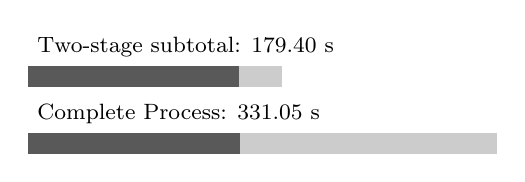
\begin{tikzpicture}[x=0.018cm,y=0.61cm,font=\footnotesize]
\fill[black!65] (0,1) rectangle (148.83,1.43);
\fill[black!20] (148.83,1) rectangle (179.40,1.43);
\node[anchor=west] at (0,1.83) {Two-stage subtotal: 179.40 s};
\fill[black!65] (0,-0.4) rectangle (149.5633,.03);
\fill[black!20] (149.5633,-0.4) rectangle (331.048,.03);
\node[anchor=west] at (0,.44) {Complete Process: 331.05 s};
\end{tikzpicture}
\caption{Historical fixed-input GEMM routing evaluation. Dark bars
show construction. The upper bar adds separate median construction
(148.83 s) and routing (30.57 s) times from different repeats.
The lower bar uses mean construction (149.56 s) and mean Process across the
same three repeats. Loading, initialization, checking, STA and output
enter only the full denominator.}
\label{fig:denominators}\end{figure}
The reservation ended during qualification. All 36 full-process and 18 construction-control timings remain missing. Figure~\ref{fig:denominators} explains why the historical construction shares of 83.0\% and 45.2\% answer different questions. To quantify the opportunity for reducing Process, let $P_r$ and $E_r$ denote Process and E2 of a reference run. Holding other stages fixed, replacing construction with $E'_r$ gives the prediction $P_r/(P_r-E_r+E'_r)$. Setting $E'_r=0$ gives the corresponding upper bound. Comparing predictions to paired Process measurements tests the fixed-remainder assumption.
\subsection{Backend Comparison: ALT CPU versus ALT CUDA}
Both backends receive the same ordered jobs and use shift 20. CPU workers own independent scratch state, whereas the GPU batches all samples and uses atomic whole-pair proposals. Their paired E2 ratio charges the GPU for preparation, transfer and synchronization. Their Process ratio also reflects downstream routing and STA. Unified backend measurements are pending.
\subsection{3D RRG Characteristics and Workload Generalization}

The XML represents vertical connectivity through resources with a layer span. All three graphs have zero edges between disjoint endpoint layer intervals. GEMM has more than twice as many nodes as either recurrent LSTM or binarized BNN. This range changes dense scratch and scan costs while keeping layer count fixed. Performance on three-layer devices remains open.
\subsection{Correctness, QoR and Applicability}\label{sec:applicability}
Auxiliary qualified maps contain 50,789, 24,434 and 23,111 changed congestion words between STRICT and ALT for GEMM, BNN and LSTM, respectively. Delay words and missing-state masks agreed in these comparisons. Changing a representative can change a route trajectory, so each route requires its own legality and QoR record. On the reserved worker, BNN Stock and Pipeline yielded identical wire maps. The ALT CPU and CUDA captures agreed across all 40 contexts, and their wire maps agreed. All four BNN routes had zero overuse and passed independent native FULL checking and STA. Each BNN log also reports 1,314 CHANZ nodes with no fan-in during graph loading. Stock and all candidates had CPD 11.0943 ns. Relative to Stock, wirelength changed by $+0.091\%$ for Pipeline and $+0.068\%$ for each ALT backend. GEMM Stock completed qualification routing, but its Pipeline invocation was interrupted. LSTM qualification and formal QoR across the three cases remain open. Valid lookahead caches remove the need for fresh construction. The GPU implementation also requires dense state for all samples to fit device memory.
